\documentclass{article}
\usepackage[a4paper]{geometry}
\usepackage{amsfonts}
\usepackage{alltt}
\usepackage{amsmath,amssymb}        % Mathpack für Formeln jeder Art
\usepackage[parfill]{parskip}       % Autoamtisch Newline, wenn Zeilenumbruch im Quelltext.
\usepackage[utf8]{inputenc}         % UTF8 Zeichensatz. 
\usepackage{xstring}				% Gebraucht für Circuitikz
\usepackage{tikz}                   % Wichtig für Zeichnungen aller Art
\input{kvmacros}                    % Kv Diagramme
\usepackage[siunitx]{circuitikz}    % Diagramme und Schaltungen
\usepackage{pgffor}
\usepackage{fancyhdr}
\usepackage{array}
\usepackage{fullpage}
\usetikzlibrary{arrows,automata}


\tikzstyle{help lines}=[blue!50,very thin]
\tikzstyle{help lines}+=[dashed]
\tikzstyle{Kreis}= [circle,draw]


\title{RS - Übung 11}
\author{Arne Beer (MN 6489196), \\
Rafael Epplee (MN 6269560)}



\begin{document}
\maketitle

\section*{Aufgabe 1}

	\begin{itemize}

	\item a) 30
	\item b) 40
	\item c) 50
	\item d) 30
	\item e) 40 

	\end{itemize}


\section*{Aufgabe 2}

	\begin{tabular}{|c|c c  c | c|} \hline
	Von&0&0&0&*\\ \hline
	Bis&1&1&0&*\\ \hline
	\end{tabular}

		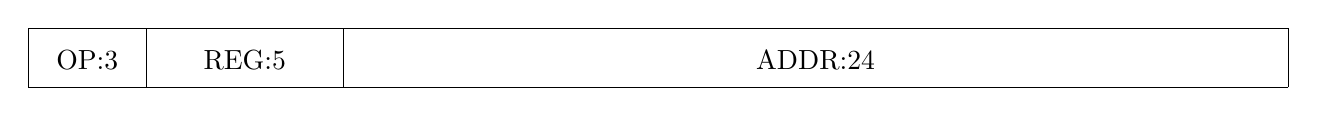
\begin{tikzpicture}
		\draw
			(0,0) -- (0,0.75) {}
	        (0,0) -- (16,0) {}
	        (0,0.75) -- (16,0.75){}
	        (16,0) -- (16,0.75){}

	        (1.5,0) -- (1.5,0.75){}
	        (4,0) -- (4,0.75){}

	        (0.75,0.35) node[] {OP:3}
	        (2.75,0.35) node[] {REG:5}
	        (10,0.35) node[] {ADDR:24}

	    ;

		\end{tikzpicture}

	\begin{tabular}{|c|c c  c | c c c c c c c | c |}\hline
	Von&1&1&1&0&0&0&0&0&0&0&*\\ \hline
	Bis&1&1&0&1&1&0&0&1&0&0&*\\ \hline
	\end{tabular}

		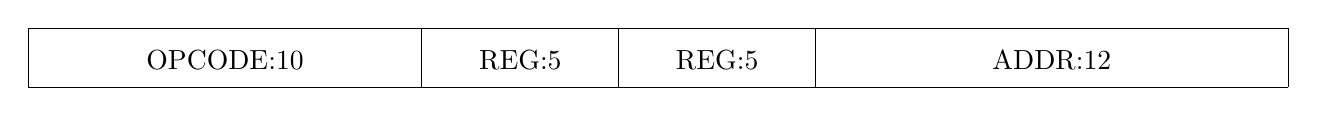
\begin{tikzpicture}
		\draw
			(0,0) -- (0,0.75) {}
	        (0,0) -- (16,0) {}
	        (0,0.75) -- (16,0.75)
	        (16,0) -- (16,0.75){}

	        (5,0) -- (5,0.75){}
	        (7.5,0) -- (7.5,0.75){}
	        (10,0) -- (10,0.75){}


	        (2.5,0.35) node[] {OPCODE:10}
	        (6.25,0.35) node[] {REG:5}
	        (8.75,0.35) node[] {REG:5}
	        (13,0.35) node[] {ADDR:12}

	        ;

		\end{tikzpicture}

	\begin{tabular}{|c|ccc|ccc|ccccc|} \hline
	Von&1&1&1&1&1&1&0&0&0&0&0\\ \hline
	Bis&1&1&1&1&1&1&1&1&1&1&0\\ \hline
	\end{tabular}

		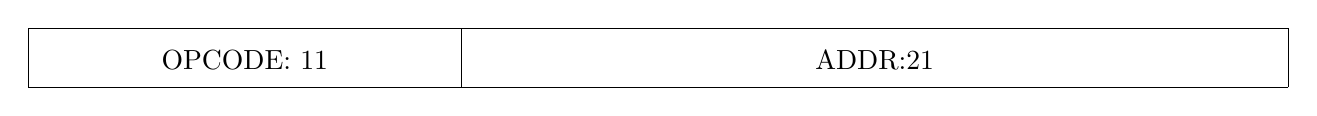
\begin{tikzpicture}
		\draw
			(0,0) -- (0,0.75) {}
	        (0,0) -- (16,0) {}
	        (0,0.75) -- (16,0.75)
	        (16,0) -- (16,0.75){}

	        (5.5,0) -- (5.5,0.75){}

	        (2.75,0.35) node[] {OPCODE: 11}
	        (10.75,0.35) node[] {ADDR:21}

	        ;

		\end{tikzpicture}

\section*{Aufgabe 3}

		\begin{itemize}

	\item a) Rot=0000 Imm8= 1011 1001
	\item b) Die Ziffer erstreckt sich über 9 Bits, kann also nicht durch imm8 dargestellt werden. 
	\item c) Nein es geht nicht, da man um 29 shiften müssten und nur um gerade Zahlen shiften kann, was durch die Multiplikation des Operators rot mit 2 bedingt ist. 
	\item d) rot=1110 Imm8=0110 0011
	\item e) rot=0010 Imm8=0000 1001

	\end{itemize}



\section*{Aufgabe 4}

	\subsection*{a)}

		\begin{itemize}
		\item 0-Adress-Maschine
			Die Befehle sind:
			\begin{verbatim}
				PUSH D
				PUSH E
				MUL
				PUSH F
				ADD
				PUSH B
				PUSH C
				MUL
				PUSH A
				SUB
				DIV
				POP R
			\end{verbatim}

		\item 1-Adress-Maschine
			Hier muss man anscheinend in den Speicher schreiben, was das ganze etwas komplizierter macht... Das folgende Programm zerstört die Werte an den Adressen D und B. Alternativ könnte man auch in neue, "unbeschriebene" Register schreiben, allerdings wissen wir nicht, ob diese für unser Programm freigegeben sind bzw. überhaupt existieren.
			\begin{verbatim}
				LOAD D
				MUL E
				ADD F
				STORE G
				LOAD B
				MUL C
				STORE H
				LOAD A
				SUB H
				DIV G
				STORE R
			\end{verbatim}

		\item 2-Adress-Maschine
			\begin{verbatim}
				MUL D,E
				ADD D,F
				MUL B,C
				SUB A,B
				DIV A,D
				MOV R,A
			\end{verbatim}

		\item 3-Adress-Maschine
			\begin{verbatim}
				LOAD G,D
				LOAD H,E
				MUL I,G,H
				LOAD G,F
				ADD H,I,G
				LOAD G,B
				LOAD I,C
				MUL J,G,I
				LOAD G,A
				SUB I,G,J
				DIV R,I,H
			\end{verbatim}
		\end{itemize}

	\subsection*{b)}
		\begin{tabular}{r | l}
			0-Adress-Maschine & $24\cdot7+5\cdot8 = 208$ Bits \\
			1-Adress-Maschine & $11\cdot24 = 264$ Bits \\
			2-Adress-Maschine & $6\cdot40 = 240$ Bits \\
			3-Adress-Maschine & $28\cdot6 + 20\cdot5 = 268$ Bits \\
		\end{tabular} \\

		Die 0-Adress-Maschine hat die kompakteste Codierung für dieses Programm.
\end{document}